\chapter{Travulog and HTravulog}{
	% Article & books
	% - A metalanguage for SystemVerilog Transformation
	\begin{comment}
		Per realizzare un'architettura FT configurabile si devono applicare le tecniche fault tolerant a tutti i blocchi dell'IF Stage e permettere poi l'applicazione o meno delle tecniche in ciascun blocco tramite dei parametri. Si è quindi deciso di creare un metalinguaggio all'interno del SystemVerilog (SV) che permetta la creazione della nuova architettura pertendo da un template e da un modulo base. Come si vede in figura \figref{fig:TravulogFlowBlocks} Questa trasformazione viene fatta da un oggetto Python collegato al template, quando si passa il modulo base all'oggetto viene creato il nuovo modulo. Questa nuova architettura è creata sulla base del template Travulog e del modulo base, essa è quindi un layer di interfaccia che rende il vecchio modulo Fault Tolerant.
		Per permettere la conversione tramite l'oggetto Travulog è necessario avere a disposizione un oggetto che contenga tutti i dati del modulo SystemVerilog associato, si è quindi creata una nuova classe Python che effettua il parsing di un file SV contenente un modulo, questa classe è stata chiamate moddata. Come mostrato in figura  \figref{fig:TravulogFlowBlocks} il file che contiene il modulo base deve essere trasformato nel corrispondente oggetto moddata e poi passato all'oggetto Travulog che genera la nuova architettura.
	\end{comment}
	To create a configurable FT architecture it is necessary to apply fault tolerant techniques to all the blocks of the IF Stage and then allow to apply or not techniques in each block by means of parameters. It was therefore decided to create a metalanguage within the SystemVerilog (SV) that allows the creation of the new architecture starting from a template and a base module, in this way we can define a template and apply it to each block of the IF stage. As you can see in figure \figref{fig:TravulogFlowBlocks} this transformation is done by a Python object linked to the template, when you pass the base module to the object the new module is created. The new FT architecture is created on the basis of the Travulog template and the base module, it is therefore an interface layer that makes the old module Fault Tolerant. 
	To allow the conversion through the Travulog object it is necessary to have an object that contains all the data of the associated SystemVerilog base module, we have therefore created a new Python class that parses a SV file containing a module, this class has been called moddata. As shown in the figure \figref{fig:TravulogFlowBlocks} the file containing the basic module must be transformed into the corresponding moddata object and then passed to the Travulog object which generates the new architecture.
	\begin{figure}[H]
		\centering
		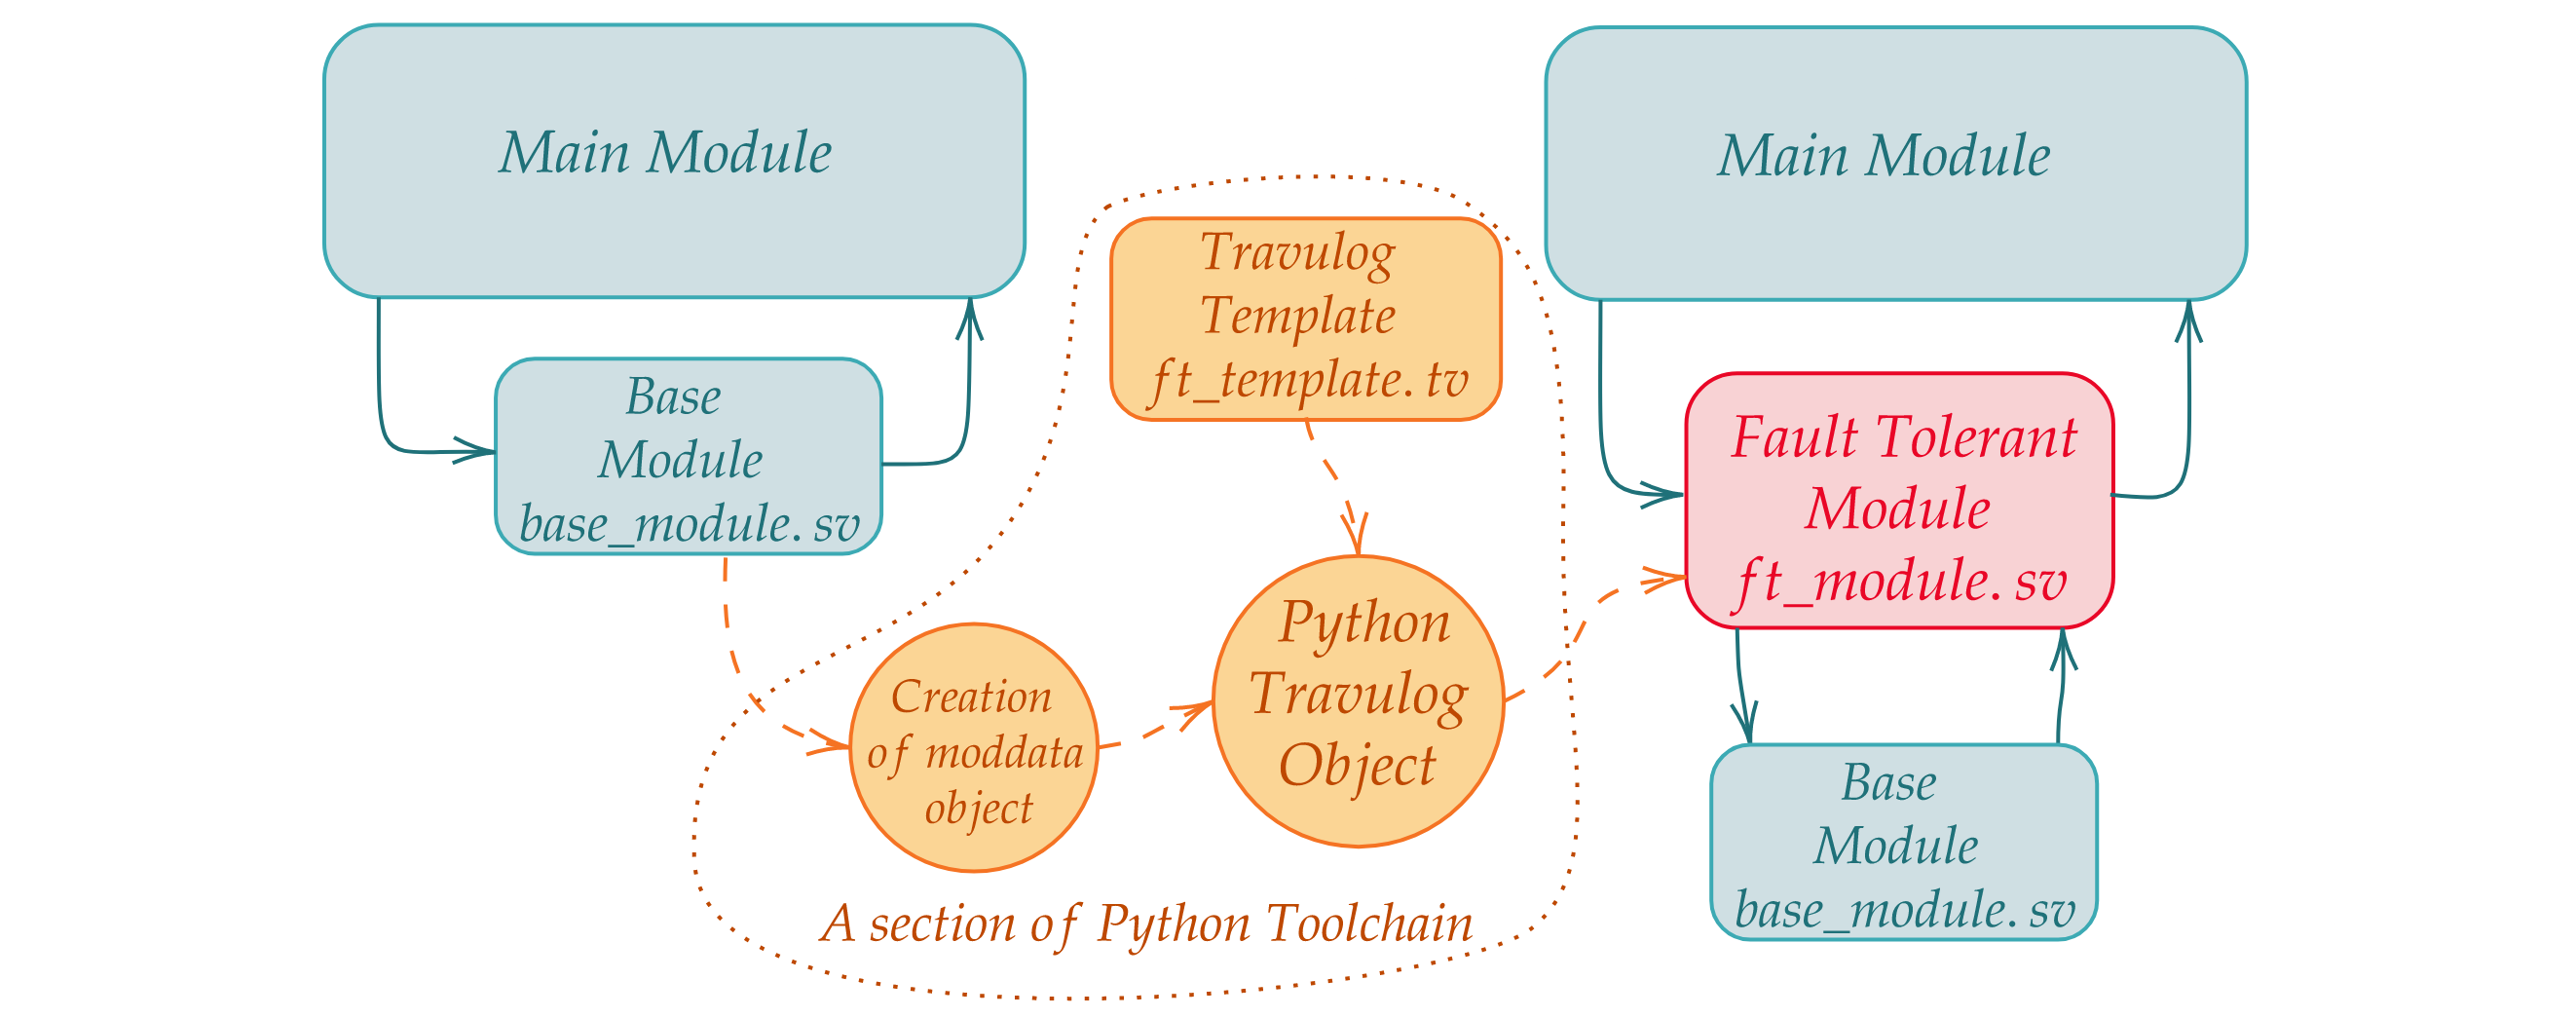
\includegraphics[scale=0.2,center]{./images/Travulog_flow_blocks.png}
		\caption{Flow diagram of architecture transformation using Travulog template}
		\label{fig:TravulogFlowBlocks}
	\end{figure} 
	
    As you can see the conversion of a SVerilog module using a Travulog template implies the use of Python code, infact you have to create the moddata object related to the Base module, the Travulog object related to the TV template and then give moddata obj to TV obj to obtain the new SV code.	
    
    For these reason, in order simplify the use of Travulog template we create the Hidden Travulog (HTV) code or HTravulog. This code is hidden inside a synthesizable SV module using four slash and a space: "//// " . 
    
    This code should be written inside the main SV module and it indicates how to apply Travulog template. Using HTV code you can also create new module from a SV block inside the current module and the apply your template to this new block. The complete functionality are described in HTravulog section. 
	
	\begin{comment}
		Per creare il nuovo linguaggio siamo partiti dal cv32e40p_compress_decoder (CD) fault tolerant e abbiamo creato una serie di comandi che permettono di creare il compress decoder FT da quello base. Analizzeremo ora i vari comandi Travulog facendo riferimento al compress decoder. 
	\end{comment}
	
	
	\section{Travulog}{
	    \label{Travulog}
    	To create the Travulog language we started from the fault tolerant cv32e40p\_compress\_decoder\_ft and we created a series of commands that allow us to create the FT compress decoder from the basic one. We will now analyze the various Travulog commands referring to the compress decoder, comparing pieces of code from the Travulog template and its conversion in SVerilog.
	
	
    	\subsection{Declaration of ports}{
    		\begin{comment}
    			Nel listato \ref{lst:declTV} è presente una parte di template Travulog, questo pezzo di codice permette di generare il System Verilog del listato \ref{lst:decl:w
    			SV}. di seguito vengono elencati i comandi in questa parte di template:
    		\end{comment}
    		In the listing \ref{lst:declTV} there is a part of the Travulog template, this piece of code allows to generate the System Verilog of the listing \ref{lst:declSV}. the commands in this part of the template are these: 
    		\begin{itemize}
    			\item [\textbf{PARAMETER\_DECLARATION}:] The command PARAMETER\_DECLARATION copy the parameter declaration from the BLOCK module in the new System Verilog module. BLOCK is an identifier used in the Travulog object that should be linked to a moddata object. Note that you can have multiple ID since ids are managed as a dictionary, e.g if you give {"BLOCK":moddata\_obj1, "BLOCK2":moddata\_obj2} to Travulog object you can use both BLOCK and BLOCK2 identifiers in the Travulog code.
    			\item [\textbf{DECLARATION\_FOREACH}:] This command cycle on the given signals and it substitute: INOUT  with "input" or "output",  BITINIT with de bits definition and SIGNAME with the name of the signal. The first argument is the module id, the second one is the type of signal: IN for input port of the module, OUT for output, IN\_OUT for both input and output and INTERN for internal signals of the module. You can also indicate some signals to exclude by the list using "NOT sig1 sig2 ... " as you can see at line 7, indeed in the example clk and rst\_n signals are excluded since they should not be triplicated.
    			This command can also be used for the declaration of internal signals and for assign statement as we see later.
    			\item [\textbf{MODULE\_NAME}:] This is a parameter that is substituted with the name given to the Travulog object, it is the name of the new module.
    		\end{itemize}
    			
    			
    		\openup -0.5em
    		
    		\begin{parcolumns}[colwidths={1=0.54\textwidth}, distance=0.5em]{2}
    			\colchunk{%
    				\begin{lstlisting}[basicstyle=\ttfamily\scriptsize, language=Verilog, caption=Declaration Travulog Code, label=lst:declTV]
module MODULE_NAME
	
	PARAMETER_DECLARATION BLOCK

(
	// compressed decoder input output
	DECLARATION_FOREACH BLOCK IN_OUT NOT clk rst_n
		INOUT logic [2:0]BITINIT SIGNAME,
	END_DECLARATION_FOREACH

	
	input logic clk,
	input logic rst_n,  
	
	// fault tolerant state
	input logic [2:0] set_broken_i,
	output logic [2:0] is_broken_o,
	output logic err_detected_o,
	output logic err_corrected_o
);
    				\end{lstlisting}
    			}
    			\colchunk{%
    				\begin{lstlisting}[basicstyle=\ttfamily\scriptsize, language=Verilog, numbers=none, caption=Declaration SVerilog code derived, label=lst:declSV]
module cv32e40p_compressed_decoder_ft
#(
	parameter FPU = 0
)
(
	// compressed decoder input output
	input  logic [2:0] [31:0] instr_i,
	output logic [2:0] [31:0] instr_o,
	output logic [2:0] is_compressed_o,
	output logic [2:0] illegal_instr_o,
	
	input logic clk,
	input logic rst_n,    
	
	// fault tolerant state
	input logic [2:0] set_broken_i,
	output logic [2:0] is_broken_o,
	output logic err_detected_o,
	output logic err_corrected_o
);
    				\end{lstlisting}
    			}
    		\end{parcolumns}
    	
    		\openup +0.5em
    		
    		
    	}% end Declaration of ports
    	
    	\subsection{Internal signals and assign}{
    		In the following listings you can see the continuation of the previous ports definition, the first "declaration\_foreach" create the signals that connect the three block outputs to the voter while the second creates block error signals. In the last two lines there is the compound parameter "SIG\_NUM-BLOCK-OUT" inside the square bracket,  this parameter is substituted in the right listing with the number (SIG\_NUM) of output ports (OUT) of the module (BLOCK) minus one, anyway instead of OUT you can use IN, PARAM, INTERN or IN\_OUT in order to have the correct signals number.
    		
    		\openup -0.5em
    		
    		\begin{parcolumns}[colwidths={1=0.5\textwidth}, distance=0.5em]{2}
    			\colchunk{%
    				\begin{lstlisting}[basicstyle=\ttfamily\scriptsize, language=Verilog, caption=Travulog Code, label=lst:internTV]
// Signals out to each compressed 
// decoder block to be voted
DECLARATION_FOREACH BLOCK OUT 
logic [2:0]BITINIT SIGNAME_to_vote ;
END_DECLARATION_FOREACH

// Error signals
DECLARATION_FOREACH BLOCK OUT 
logic [2:0] SIGNAME_block_err ; 
END_DECLARATION_FOREACH

// Signals that use error signal to 
// find if there is one error on each 
// block, it is the or of previous signals
logic [2:0] block_err_detected;
logic [SIG_NUM-BLOCK-OUT:0] err_detected;
logic [SIG_NUM-BLOCK-OUT:0] err_corrected;
    				\end{lstlisting}
    			}
    			\colchunk{%
    				\begin{lstlisting}[basicstyle=\ttfamily\scriptsize, language=Verilog, numbers=none, caption=SVerilog code derived, label=lst:internSV]
// Signals out to each compressed 
// decoder block to be voted
logic [2:0] [31:0] instr_o_to_vote ;
logic [2:0] is_compressed_o_to_vote ;
logic [2:0] illegal_instr_o_to_vote ;

// Error signals
logic [2:0] instr_o_block_err ;
logic [2:0] is_compressed_o_block_err ;
logic [2:0] illegal_instr_o_block_err ;

// Signals that use error signal to 
// find if there is one error on each 
// block, it is the or of previous signals
logic [2:0] block_err_detected;
logic [2:0] err_detected;
logic [2:0] err_corrected;
    				\end{lstlisting}
    			}	
    		\end{parcolumns}
    
    		\openup +0.5em
    	
    	} % end Internal signals and assign
    	
    	\subsection{Instance}{
    		\begin{comment}
    			Per poter creare una nuova instanza da un blocco esistente è stato creato il comando INSTANCE mostrato nel listing \ref{lst:instance1TV}. Dopo la keyword INSTANCE dev'essere indicato l'id del blocco e il nome della nuova instanza che verrà creata, come è mostrato nel listing seguente per creare il nome della nuova instanza viene utilizzato il parametro BLOCK_MODNAME, questo è sostituito in fase di preprocessamento con il nome del modulo a cui l'id BLOCK è riferito.
    			Successivamente all'interno del comando vengono indicate le connessioni da effettuare. PARAM si riferisce ai parametri e il comando a riga due indica di connettere i parametri allo stesso nome, infatti si ha .FPU(FPU). A riga 3 invece viene indicato di connettere i segnali clk e rst_n a stesso nome, la riga successiva connette gli ingressi al loro stesso nome ma aggiungendo il suffisso "[0]", dagli ingressi però vengono esclusi i segnali già connessi nell'if precedente. Nella conversione in SV che vedete sulla destra non sono presenti il clock e il reset quindi il comportamento indicato sopra non è evidente.
    			Come già accennato le connessioni all'interno del comando INSTANCE sono sensibili all'ordine in cui vengono fatte, percui per esempio gli IF sugli ingressi vanno fatti prima di assegnare genericamente gli ingressi con "IN = IN" altrimenti gli if non sono considerati. Stessa considerazione per le uscite e i parametri.
    		\end{comment}
    
            In order to create a new instance from an existing block,  was created the INSTANCE command shown in the listing \ref{lst:instance1TV}. After the INSTANCE keyword, there are the block id and the name of the new instance. As shown in listing \ref{lst:instance1TV} the BLOCK\_MODNAME parameter is used to create the name of the new instance, this parameter is replaced in the preprocessing phase with the name of the BLOCK module.
            
            The connection commands are indicated inside the INSTANCE command. The command at line two indicates to connect the parameters to the same name, in fact we have .FPU (FPU). At line 3 instead it is indicated to connect clk and rst\_n signals to the same name, the next line connects the inputs to their same name but it adds the suffix "[0]", however, at the signals already connected in the previous if are not appended the suffix. In the conversion to SV on the right there are no clocks and no reset so the behavior just described is not evident.
            
            As already mentioned, the connections inside the INSTANCE command are sensitive to the order in which they are made, for example the IF on the inputs should be before assigning the inputs generically with "IN = IN", otherwise the ifs are not considered. Same consideration for outputs and parameters. 
        
    		\openup -0.5em
    	
    		\begin{parcolumns}[colwidths={1=0.5\textwidth}, distance=0.5em]{2}
    		\colchunk{%
    			\begin{lstlisting}[basicstyle=\ttfamily\scriptsize, language=Verilog, caption=Instance Travulog Code, label=lst:instance1TV]
INSTANCE BLOCK BLOCK_MODNAME_no_ft
PARAM=PARAM
IF clk rst_n IN=IN
IN= IN[0]
OUT = OUT[0]
END_INSTANCE
    
    
    
    
    
    	
    	
    	
    	
    	
    			\end{lstlisting}
    		}
    		\colchunk{%
    			\begin{lstlisting}[basicstyle=\ttfamily\scriptsize, language=Verilog, numbers=none, caption=Instance SVerilog code derived, label=lst:instance1SV]
cv32e40p_compressed_decoder
#(
    .FPU (FPU)
)
compressed_decoder_no_ft
(
    // Input ports of compressed_decoder_no_ft
    .instr_i                (  instr_i[0]),

    // Output ports of compressed_decoder_no_ft
    .instr_o        (  instr_o[0]),
    .is_compressed_o(  is_compressed_o[0] ),
    .illegal_instr_o(  illegal_instr_o[0] )
);		
    			\end{lstlisting}
    		}	
    		\end{parcolumns}
    	
    		\openup +0.5em
    		
        	
        	In the cv32e40p\_compressed\_decoder\_ft module there are as many conf\_voter as the output of the cv32e40p\_compressed\_decoder (CD), infact the CD is triplicated and we need a conf\_voter for each output. In order to automatize the creation and the connection of the conf\_voter we create the command INSTANCE\_FOREACH. After this keyword there is the id of the block and the list of signals on which cycle on. It can be used IN, OUT, IN\_OUT and INTERN as abbreviation for the list, in this way the code is compressed and clearer.
        	
        	
        	As just mentioned INSTANCE\_FOREACH cycles on the signals list and it substitutes in the verilog code: BITNUMBER with the number of bits of the signal, INDEX with the current cycle number and SIGNAME with the name of the signal.
        
        	In the listing below you can see an example of how the INSTANCE\_FOREACH command works.
        	
    		\openup -0.5em
    	
    		\begin{parcolumns}[colwidths={1=0.5\textwidth}, distance=0.5em]{2}
    		\colchunk{%
    			\begin{lstlisting}[basicstyle=\ttfamily\scriptsize, language=Verilog, caption=Instance  foreach  Travulog  Code, label=lst:instance2TV]
INSTANCE_FOREACH BLOCK OUT    
    // Voter for TOVOTE signal, triple voter if
    // PARAM_NAME_TOUT[INDEX] == 1
    cv32e40p_conf_voter
    #(
        .L1(BITNUMBER),
        .TOUT(PARAM_NAME_TOUT[INDEX])
    ) voter_SIGNAME_INDEX
    (
        .to_vote_i( SIGNAME_to_vote ),
        .voted_o( SIGNAME),
        .block_err_o( SIGNAME_block_err),
        .broken_block_i(is_broken_o),
        .err_detected_o(err_detected[INDEX]),
       .err_corrected_o(err_corrected[INDEX])
    );
END_INSTANCE_FOREACH
    
    
    
    
    
    
    
    
    
    
    
    
    
    
    
    
    
    
    
    
    
    
    
    
    
    
    
    
    
    			\end{lstlisting}
    		}
    		\colchunk{%
    		    \begin{lstlisting}[basicstyle=\ttfamily\scriptsize, language=Verilog, numbers=none, caption=Instance foreach SVerilog code , label=lst:instance2SV]
// Voter for TOVOTE signal, triple voter if
 // CODE_TOUT[0] == 1
cv32e40p_conf_voter
#(
    .L1(32),
    .TOUT(CODE_TOUT[0])
) voter_instr_o_0
(
    .to_vote_i( instr_o_to_vote ),
    .voted_o( instr_o),
    .block_err_o( instr_o_block_err),
    .broken_block_i(is_broken_o),
    .err_detected_o(err_detected[0]),
    .err_corrected_o(err_corrected[0])
);
// Voter for TOVOTE signal, triple voter if
// CODE_TOUT[1] == 1
cv32e40p_conf_voter
#(
    .L1(1),
    .TOUT(CODE_TOUT[1])
) voter_is_compressed_o_1
(
    .to_vote_i( is_compressed_o_to_vote ),
    .voted_o( is_compressed_o),
    .block_err_o( is_compressed_o_block_err),
    .broken_block_i(is_broken_o),
    .err_detected_o(err_detected[1]),
    .err_corrected_o(err_corrected[1])
);
// Voter for TOVOTE signal, triple voter if
// CODE_TOUT[2] == 1
cv32e40p_conf_voter
#(
    .L1(1),
    .TOUT(CODE_TOUT[2])
) voter_illegal_instr_o_2
(
    .to_vote_i( illegal_instr_o_to_vote ),
    .voted_o( illegal_instr_o),
    .block_err_o( illegal_instr_o_block_err),
    .broken_block_i(is_broken_o),
    .err_detected_o(err_detected[2]),
    .err_corrected_o(err_corrected[2])
);
    			\end{lstlisting}
    		}	
    		\end{parcolumns}
    	
    		\openup +0.5em
    		
    	} % end instance
    
    	\subsection{Multiple Operation}{
            An instance of compressed\_decoder have an error if there is at least an output signal wrong, for these reason error\_detected signals is found by applying OR operation between *\_block\_err signals out of the conf\_voters. The number of *\_block\_err signals is equal to the number of output of the module used, in this case the three output of the compressed\_decoder, for this reason we create the Travulog command OP\_FOREACH that apply a logic operation to a set of signals. 
            
            After the keyword OP\_FOREACH there should be the module id and then the signals identifier (IN, OUT, IN\_OUT, INTERN, PARAM), these two element identify the list of signals to cycle on. Then there should be the operation to apply ( |, \& etc ) and the pattern to use for each signal ( SIGNAME will be replaced with the name of the signal).
            
            In the listing \ref{lst:multiopTV} is applied a  suffix to the signame in order to apply OR to correct block\_err signals, instead in the right listing there is the conversion of Travulog code, each TV line becomes three lines of SV. 
    	
    		\openup -0.5em
    	
    		\begin{parcolumns}[colwidths={1=0.5\textwidth}, distance=0.5em]{2}
    		\colchunk{%
    			\begin{lstlisting}[basicstyle=\ttfamily\scriptsize, language=Verilog, caption=Instance  foreach  Travulog  Code, label=lst:multiopTV]
assign block_err_detected[0] = OP_FOREACH BLOCK OUT | SIGNAME_block_err[0] ; 


assign block_err_detected[1] = OP_FOREACH BLOCK OUT | SIGNAME_block_err[1] ; 


assign block_err_detected[2] = OP_FOREACH BLOCK OUT | SIGNAME_block_err[2] ; 



        		\end{lstlisting}
    		}
    		\colchunk{%
    		    \begin{lstlisting}[basicstyle=\ttfamily\scriptsize, language=Verilog, numbers=none, caption=Instance foreach SVerilog code , label=lst:multiopSV]
assign block_err_detected[0] =  
          instr_o_block_err[0]
        | is_compressed_o_block_err[0]
        | illegal_instr_o_block_err[0]; 
assign block_err_detected[1] =  
          instr_o_block_err[1]
        | is_compressed_o_block_err[1]
        | illegal_instr_o_block_err[1]; 
assign block_err_detected[2] =  
          instr_o_block_err[2]
        | is_compressed_o_block_err[2]
        | illegal_instr_o_block_err[2]; 

    			\end{lstlisting}
    		}	
    		\end{parcolumns}
	
    		\openup +0.5em
        	
    	}% end Multiple Operation 
    	
    	\subsection{Converted SV and parameters template}{
            At the end of the Travulog conversion you will obtain the cv32e40p\_compressed\_decoder\_ft.sv file (listing \ref{lst:cdftSV} ) containing an architecture layer that makes the cv32e40p\_compressed\_decoder fault tolerant.
            
    		\openup -0.5em
    	
        	\lstinputlisting[basicstyle=\ttfamily\scriptsize, language=Verilog, caption=Fault Tolerant compressed decoder layer, label=lst:cdftSV]{./code/cv32e40p_compressed_decoder_ft.sv}
        	
    		\openup +0.5em
    		
    		This SVerilog architecture needs some parameters: CODE\_FT, CODE\_TIN,
    		
    		CODE\_TOUT,  CODE\_DECREMENT,  CODE\_INCREMENT,     
    		
    		CODE\_BREAKING\_THRESHOLD,     
    		CODE\_COUNT\_BIT, CODE\_INC\_DEC\_BIT. 
    		
    		These parameters are contained in the cv32e40p\_pkg2 package imported at line one of listing \ref{lst:cdftSV}, the creation of this package can be automatized using a parameters template, for example our fault tolerant TV template ft\_template.sv needs its TV parameters template ft\_template\_parameters.sv, this template is shown in listing \ref{lst:paramTV}.
    		
    		
    		\openup -0.5em
    	
        	\lstinputlisting[basicstyle=\ttfamily\scriptsize, language=Verilog, caption=Parameters template for Fault tolerant module, label=lst:paramTV]{./code/ft_template_parameters.sv}
        	
    		\openup +0.5em
    		
    		
    		
    	}% end parameters template
    	
    	\subsection{Apply the template in Python}{
            In order to apply the Travulog template to a module you can use HTravulog code where the module is instanced or you can directly use Python code. In this section we follow the second way and so we explain how Python code is structured and how to use it.
            
            The whole code of the toolchain is in the \url{https://github.com/Elia1996/Travulog} repository, so you can clone it and use it. 
            
            In order to use Travulog template you need the files \textit{moddata.py} and \textit{travulog.py}, the first file contains many functions and the moddata class that enable the parsing an manipulation of a SVerilog module, instead the second file contains the travulog class.
            
            If you want to apply a Travulog template, the faster way is to look at test\_travulog.py file reported below.
            \begin{lstlisting}[basicstyle=\ttfamily\scriptsize, language=Python, caption=Basic Python code to use Travulog, label=lst:texttravulog]
#!/usr/bin/python3
from travulog import *

template_fname = "templates/ft_template.sv"
template_params_fname = "templates/ft_template_parameters.sv"
module_fname_dict = {"BLOCK" : "./test/arch/cv32e40p_compressed_decoder.sv"}
module_prefix = "cv32e40p_"

tr = travulog(template_fname, template_params_fname, module_fname_dict, module_prefix)

print(tr.GetElaboratedTemplate("New_module_name","PARAM_NAME"))
print(tr.GetElaboratedTemplateParams("New_module_name","PARAM_NAME"))
            \end{lstlisting}
            
            As you can see after the import of the travulog module are defined some parameters: 
            \begin{itemize}
                \item \textbf{template\_fname:} this is the fault tolerant template written in Travulog, the extension is irrelevant.
                \item \textbf{template\_params\_fname:} this is the TV template of parameters, it is used at line twelve where it is converted according to the current module name that in our case is the compressed\_decoder,
                \item \textbf{module\_fname\_dict:} This is a dictionary that connects module ids with corresponding module SVerilog filename. In this case BLOCK is connected to the compressed\_decoder filename and for this reason the Travulog object create the fault tolerant compressed decoder. Anyway you can have multiple module ids, you only need to set it in this dictionary.
                \item \textbf{module\_prefix:} This should be the prefix of each filename and module name, it should always end with a  "\_" character and it is used to create correct parameter base name.
            \end{itemize} 
            
            Once created the travulog object using these parameters, you can use GetElaboratedTemplate function to create the new cv32e40p\_compressed\_decoder\_ft.sv file text and you can use GetElaboratedTemplateParams function to create the parameters initialization for the package.
            For directly use the new architecture you should create a new package file containing the parameters initialization and import this package in the new ft module.
        
        }
    
    The way in which has been structured the Python code enable the creation of new powerful Travulog commands, so the TV commands analyzed is only a small example of what can be done using this tool since TV code can be extended according to your architectural needs. 
	}% end RISCV 32bit ISA 


	\section{Hidden Travulog}{
        As already mentioned, Hidden Travulog or HTV is a particular comment code inside a SVerilog file, the difference respect to a comment is the "//// " beginning key (HTKEY) instead of "//". The HTV parser only analyze the code after the HTKEY so be careful to correcty write "//// " before the HTV code.
        
        The result of a hidden code as HTV is the higher architecture maintenance, indeed the SVerilog architecture can be simulated, synthesised and modified with HTV code. After that a change in the base arch is done you can proceed with the HTravulog conversion, at the end of the process you obtain a new architecture that contains the base architecture changes. This maintenance process is shown in figure \ref{fig:HtravulogCycle}.
		\begin{figure}[H]
			\centering
			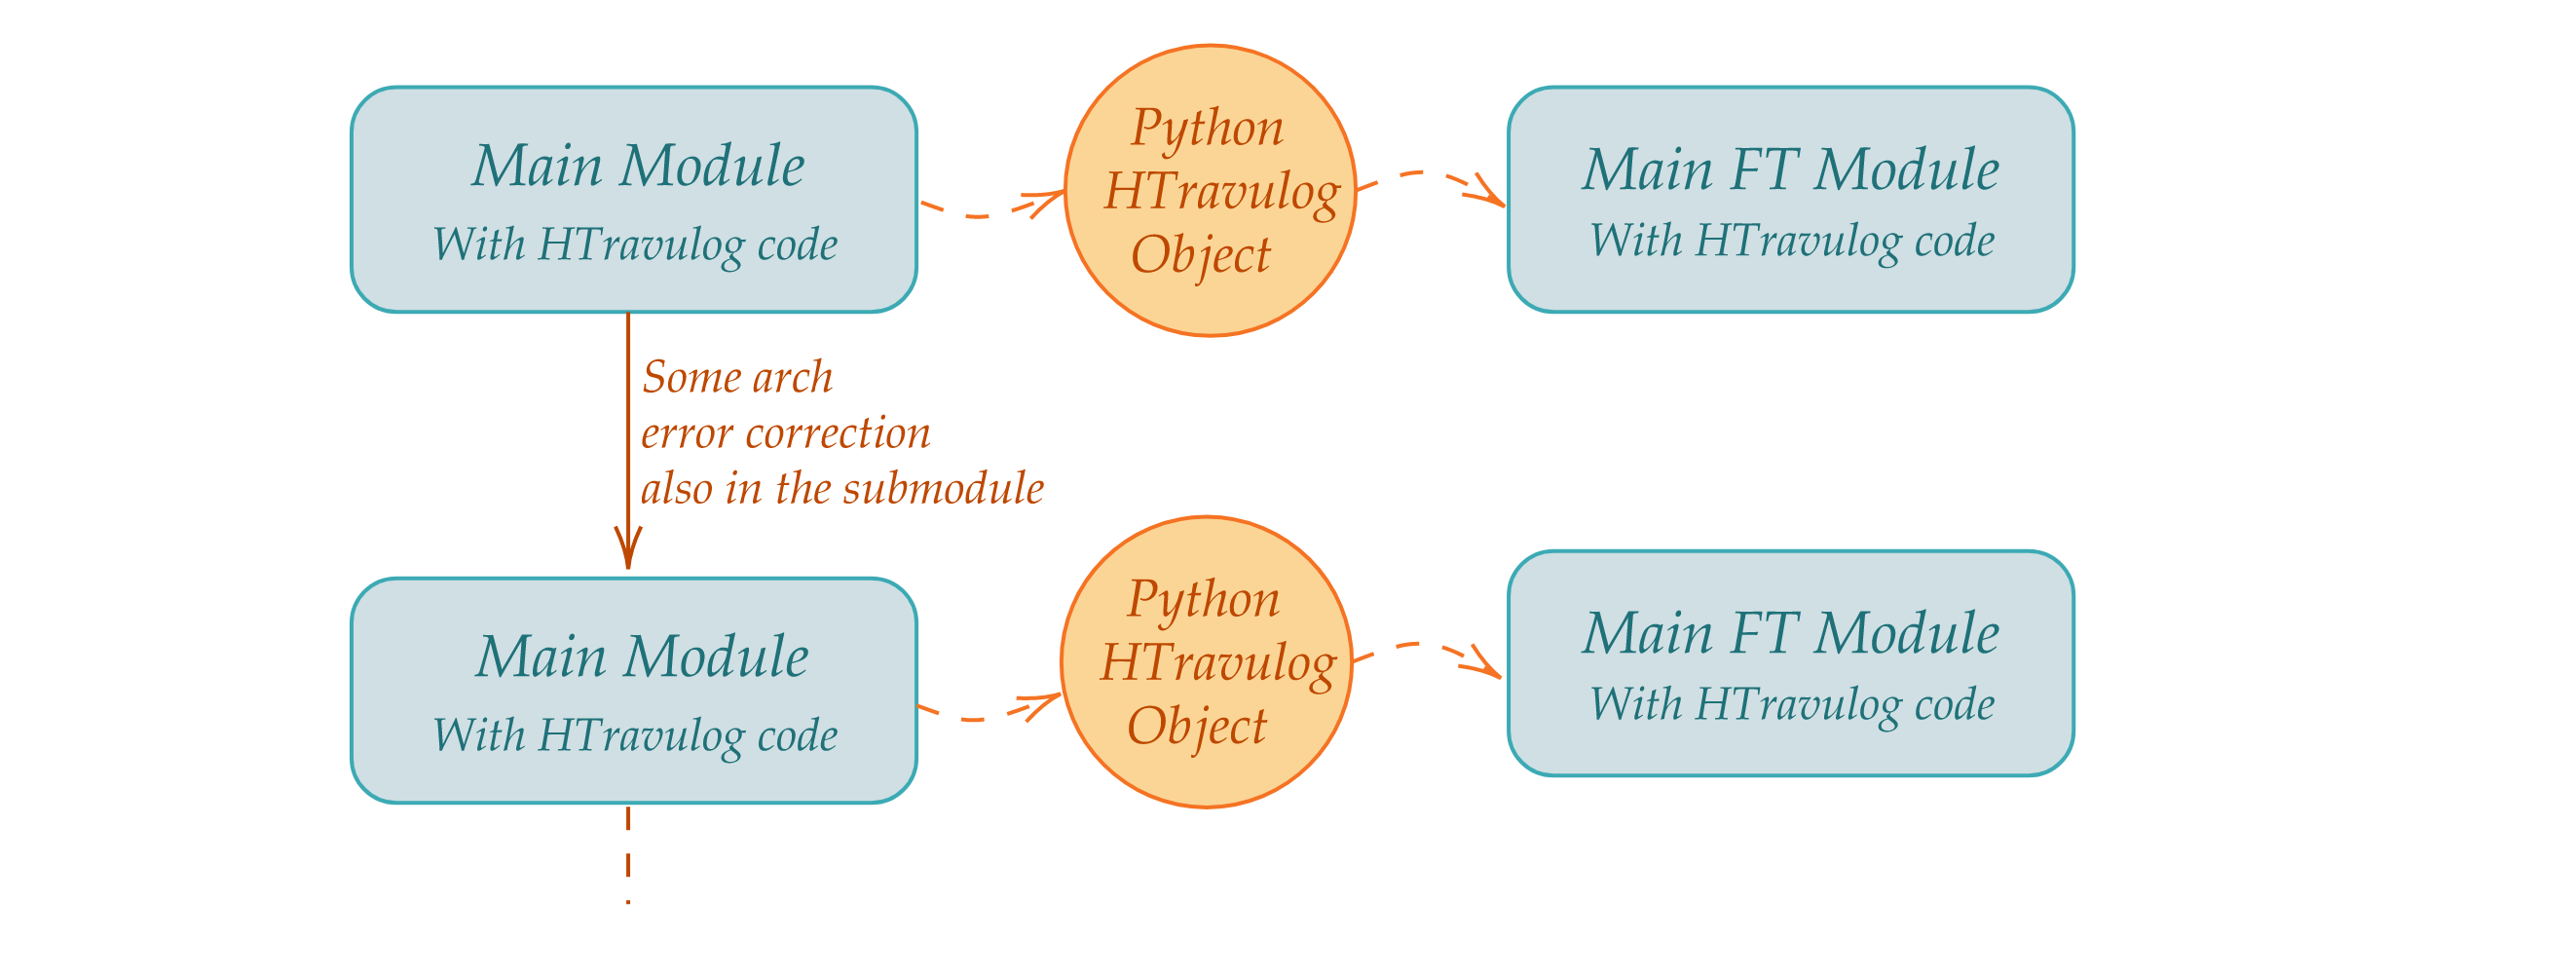
\includegraphics[scale=0.2,center]{./images/HTravulogArchMaintenance.png}
			\caption{HTravulog used during architecture life cycle}
			\label{fig:HtravulogCycle}
		\end{figure} 
        
        For the purpose of this Master Thesis are created only few HTV commands that can be extended for other uses. Anyway at this implementation step, HTV code can be used inside a whatever SVerilog module for these purpose:
        \begin{itemize}
            \item \textbf{Add some line:} The command ADD\_LINE allows to add an arbitrary line to the converted architecture.
            \item \textbf{Change internal signals:} The command FOREACH allows to cycle on input, output, internal signals and parameters in order to use their name for some connection or declaration.
            \item \textbf{Create new module:} When you want to apply a Travulog template to a piece of your \textit{architecture A} but it is written as a part of the module, you can use CREATE\_MODULE command. With this command you can transform the piece of \textit{arch A} in a new \textit{module B} written in a new SV file, additionally the command automatically creates the instance of \textit{module B} in the converted \textit{architecture A}. 

            \item \textbf{Apply a Travulog template to a module:} In the main module of an architecture you normally have many instances of modules, for each instance you can use ADD\_MODULE\_LAYER. This commmand transforms the instanced module using a Travulog template and it create the new correct instance.
        \end{itemize}
        
        These are the main transformation you can apply with HTravulog code.
        
        Now in order to explain how HTV parser works we divide SVerilog module in these four sections:
        
        \begin{itemize}
            \item \textbf{Introduction:} It is the SV code from the beginning of the file up to the module declaration, here you usually import package and you write the architecture license. In this section you can use these HTV commands: IMPORT, ADD\_LINE, NEW\_MODULE\_NAME and  NEW\_MODULE\_FILE. These command are explained in \ref{Introduction} section.
            
            \item \textbf{Port declarations:} In this section are defined the input and output of the module, at the moment this section can't be modified in order to maintain the same interface, anyway the code is organized in order to simplify the extension of HTV code also in this section.
            
            \item \textbf{Intern signals and assign:} This section starts at the end of port declaration and ends with the command "END\_DECLARATIONS", In this section you should define all intern signals and all assignment that you what to change during conversion. Just before the begin of the architecture structure definition you should place the "END\_DECLARATIONS" command in order to notify the tool that the third section ends. This section is analyzed in \ref{InternalSignals} section.
            
            In this section you can use only the command FOREACH.
            
            \item \textbf{Architecture definition:} This section starts after the  "END\_DECLARATIONS" command and ends with the module. Here you can use CREATE\_MODULE and ADD\_MODULE\_LAYER commands, these are two powerful commands that are described in section \ref{CreateNewModule} and \ref{AddModuleLayer}.
            
        \end{itemize}
        
        In the following section we analyze each section and command in detail.
        
        \subsection{Introduction}{
            \label{Introduction}
            This is the section of code before the declaration of the module, in listing \ref{lst:ifstageIntro} there is an example of SV mixed with HTV code used in cv32e40p\_if\_stage.sv
            file.
            \begin{lstlisting}[basicstyle=\ttfamily\scriptsize, language=Verilog, caption=Introduction of cv32e40p if stage, label=lst:ifstageIntro]
//// IMPORT htv_pkg.tv

import cv32e40p_pkg::*;
//// ADD_LINE import cv32e40p_pkg2::*;

//// NEW_MODULE_NAME cv32e40p_if_stage
//// NEW_MODULE_FILE OUT_DIR/cv32e40p_if_stage_ft.sv
            \end{lstlisting}
           
            At line one there is the IMPORT command used to import a parameters file, this file is parsed by the tool in order to import some parameters. In listing \ref{lst:htvpkg} there is an example of \textit{htv\_pkg.tv} file, all parameter are mandatory. BASEDIR is an abbreviations of the complete base path, we use BASEDIR for space reasons but the real file contain the complete path. 
            
            \begin{lstlisting}[basicstyle=\ttfamily\scriptsize, language=Verilog, caption=Introduction of cv32e40p if stage, label=lst:htvpkg]
IN_DIR BASEDIR/test/arch
OUT_DIR BASEDIR/out
TEMPLATE ft_template
        FILE BASEDIR/templates/ft_template.sv
        PARAM_FILE BASEDIR/templates/ft_template_parameters.sv
END_TEMPLATE
PKG_FILE BASEDIR/templates/cv32e40p_pkg2.sv
PKG_OUT_FILE BASEDIR/out/cv32e40p_pkg2.sv
MODULE_PREFIX cv32e40p_
            \end{lstlisting}
            
            The first two line set IN\_DIR and OUT\_DIR, these two parameters can be used in the main file as abbreviations of the corresponding directory set. Usually you set IN\_DIR as the directory where there is all base architecture and OUT\_DIR as the directory where you want to save the transformed architecture.
            
            The TEMPLATE statement is a command that you should use to define Travulog templates, right after TEMPLATE there is the \textit{template id} that you will use in HTV code, in the next line is defined the Travulog file of the template with the FILE key and at line five is defined the parameters template file with the PARAM\_FILE key. The TEMPLATE statement terminate with the keyword END\_TEMPLATE at line six, anyway in this file there is the possibility to define multiple template id using the structure defined before.
            
            
            Line seven and eight set the package template file and the output package file,  
            
            \begin{lstlisting}[basicstyle=\ttfamily\scriptsize, language=Verilog, caption=Introduction of cv32e40p if stage, label=lst:htvpkg2]
//// IMPORT htv_pkg.tv
    .
    .
    .
//// ADD_MODULE_LAYER 
//// TEMPLATE ft_template 
//// INFILE IN_DIR/cv32e40p_prefetch_buffer.sv
//// OUTFILE OUT_DIR/cv32e40p_prefetch_buffer_ft.sv
    .
    verilog instance
    .
//// END_ADD_MODULE_LAYER
            \end{lstlisting}
        
        }% end Before the main module declaration
        \subsection{Internal signals}{
            \label{InternalSignals}
        
        }% end internal signals
        \subsection{Create a new module}{
            \label{CreateNewModule}
        
        }% end create a new module
        \subsection{Use Travulog template}{
            \label{AddModuleLayer}
        
        }% end use travulog template 
	}% end of Architecture of CV32E40P
	
	\section{V}{
		
	}% end of Verification of CV32E40P core

	\section{CV32E40P core in Pulpissimo}{
		
	}% end of CV32E40P core in Pulpissimo

}
